\documentclass[12pt, a4paper]{article}

% 引入宏包
\usepackage[UTF8]{ctex} % 中文支持
\usepackage{geometry} % 边距设置
\geometry{left=2.5cm, right=2.5cm, top=3cm, bottom=3cm}
\usepackage{graphicx} % 插入图片
\usepackage{float} % 强制图片位置
\usepackage{caption} 
\usepackage{subcaption} % 并排子图
\usepackage{color}
\usepackage{hyperref}
\usepackage{fancyhdr}

% 设置超链接
\hypersetup{colorlinks=true, linkcolor=black, urlcolor=blue}

% 页眉页脚
\pagestyle{fancy}
\setlength{\headheight}{15pt} % 修复页眉高度警告
\fancyhf{}
\fancyhead[L]{电子电路CAD与设计}
\fancyhead[R]{硬件PCB设计报告}
\fancyfoot[C]{\thepage}

\begin{document}

% ---------------- 封面 ----------------
\begin{titlepage}
    \begin{center}
        \vspace*{2cm}
        \Huge{\textbf{智能自适应流水灯控制系统设计}}\\
        \vspace{0.5cm}
        \Large{\textbf{PCB原理图绘制 2026.6.2}}\\
        \vspace{2cm}
        
        \large
        \begin{tabular}{rl}
            \textbf{课程名称：} & 电子电路设计与仿真 \\
            \textbf{学生姓名：} & [姓名] \\  % <--- 这里改成你的名字
            \textbf{学号：} & [学号] \\      % <--- 这里改成你的学号
            \textbf{完成日期：} & \today \\
        \end{tabular}
        \vspace{3cm}
        
        \rule{0.8\textwidth}{0.5pt} \\
        \vspace{0.5cm}
        \textit{本项目以CD4017与555定时器为基础构建流水灯硬件架构。为提升系统的工程实用价值，分别通过引入模拟传感器实现\textbf{环境联动报警}，以及引入微控制器（MCU）实现\textbf{PWM呼吸算法}与\textbf{UART串口通信}，完成了具有较高复杂度的物联网控制系统原型设计}
    \end{center}
\end{titlepage}

\newpage
\tableofcontents % 自动生成目录
\newpage
% ---------------- 正文 ----------------

\section{设计任务与工程需求分析}
本次实验的主要任务是将前期在 Multisim/Tinkercad 中验证成功的虚拟电路，转化为能够实际生产打样的物理电路板（PCB）



\subsection{传感器与时钟回路}
使用 NE555 芯片搭建多谐振荡器，留出了 2.54mm 间距的排针接口（U4），用于外接 \textbf{NTC 热敏电阻}。通过这种设计，当环境温度升高导致 NTC 阻值下降时，555 定时器的充放电周期缩短，输出频率升高，实现了温度越高流水越快的视觉报警功能

\subsection{软硬件跳线接口}
为满足系统与MCU联动的需求，我在 555 定时器输出端（引脚3）与 CD4017 时钟输入端（引脚14）之间插入了一个 3P 选通排针（H1）
\begin{itemize}
    \item \textbf{硬件} 用跳线帽短接 1、2 引脚，CD4017 时钟由板载 555 芯片提供
    \item \textbf{MCU 扩展} 拔下跳线帽，将单片机的 PWM 引脚接入排针第 3 脚。此时板载 555 芯片被隔离，流水灯的跑动速度、呼吸亮度由外部代码控制
\end{itemize}

\begin{figure}[H]
    \centering
    % 请确保上传了原理图截图，命名为 schematic.png
    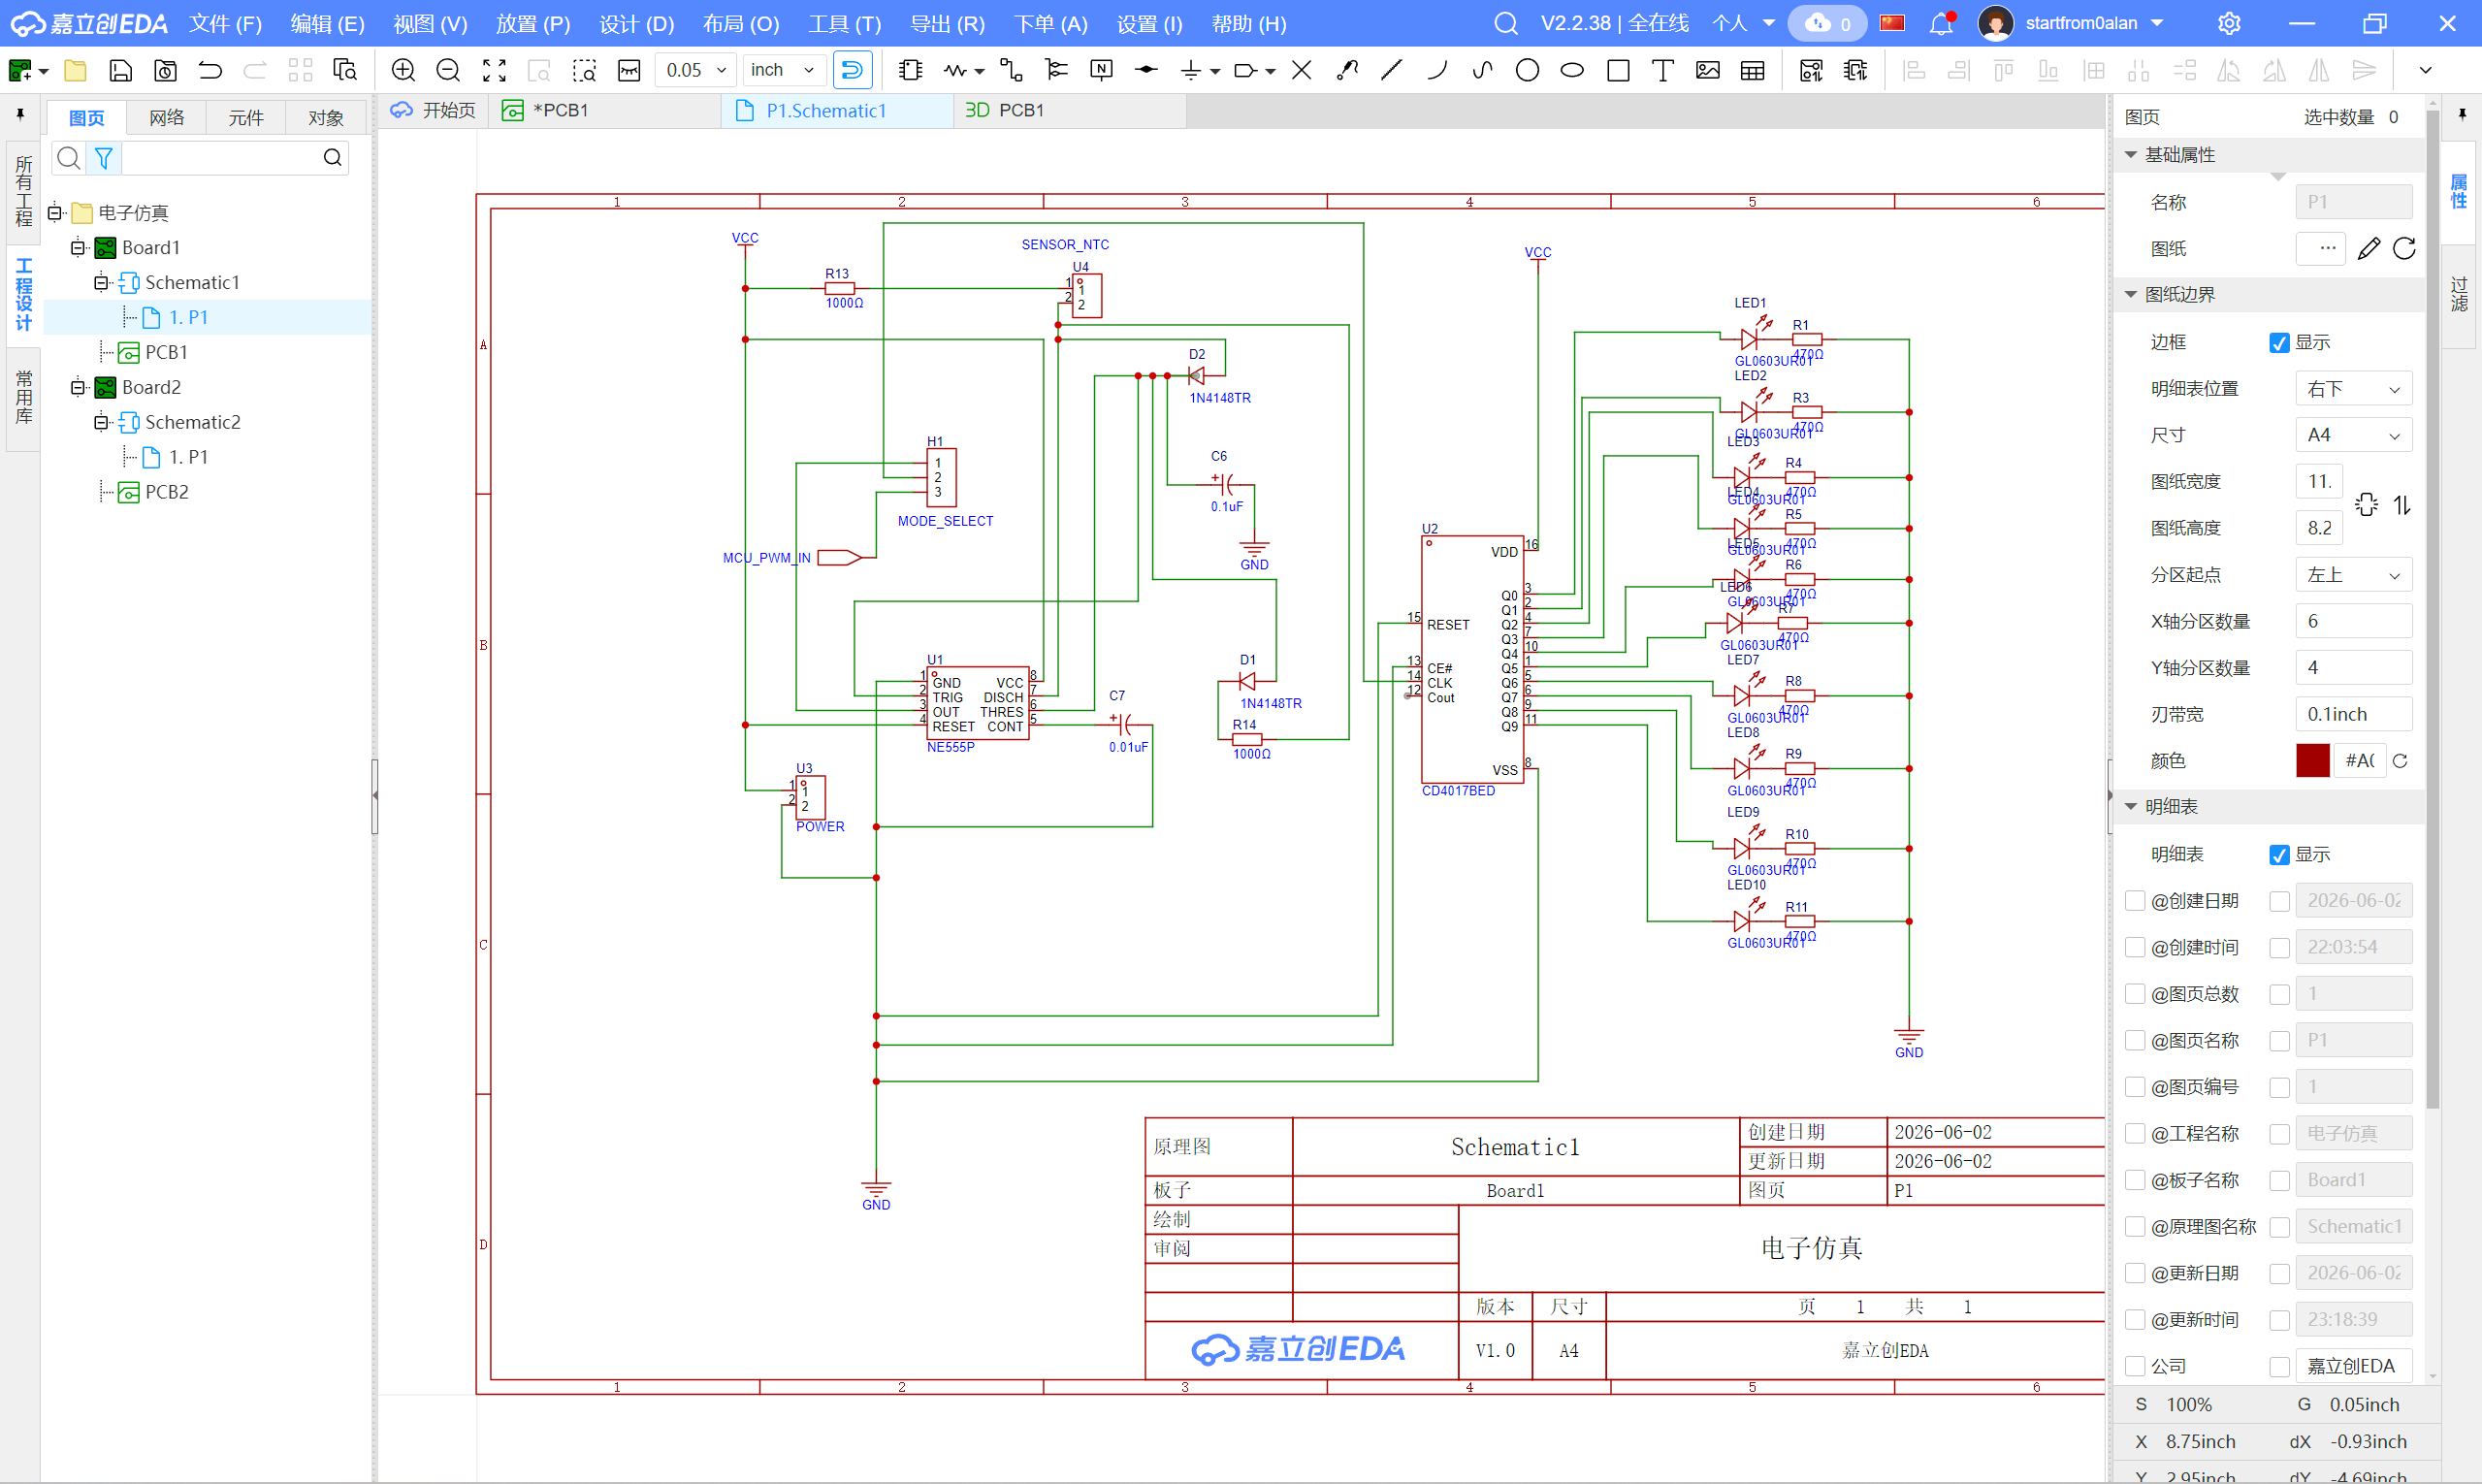
\includegraphics[width=\textwidth]{schematic.png}
    \caption{原理图}
    \label{fig:schematic}
\end{figure}

\section{PCB 布局布线与 3D 可视化验证}
在原理图无 DRC 报错后导入至 PCB 环境进行物理层面的布局与走线

\begin{figure}[H]
    \centering
    % 请确保上传了 2D 走线图，命名为 pcb_2d.png
    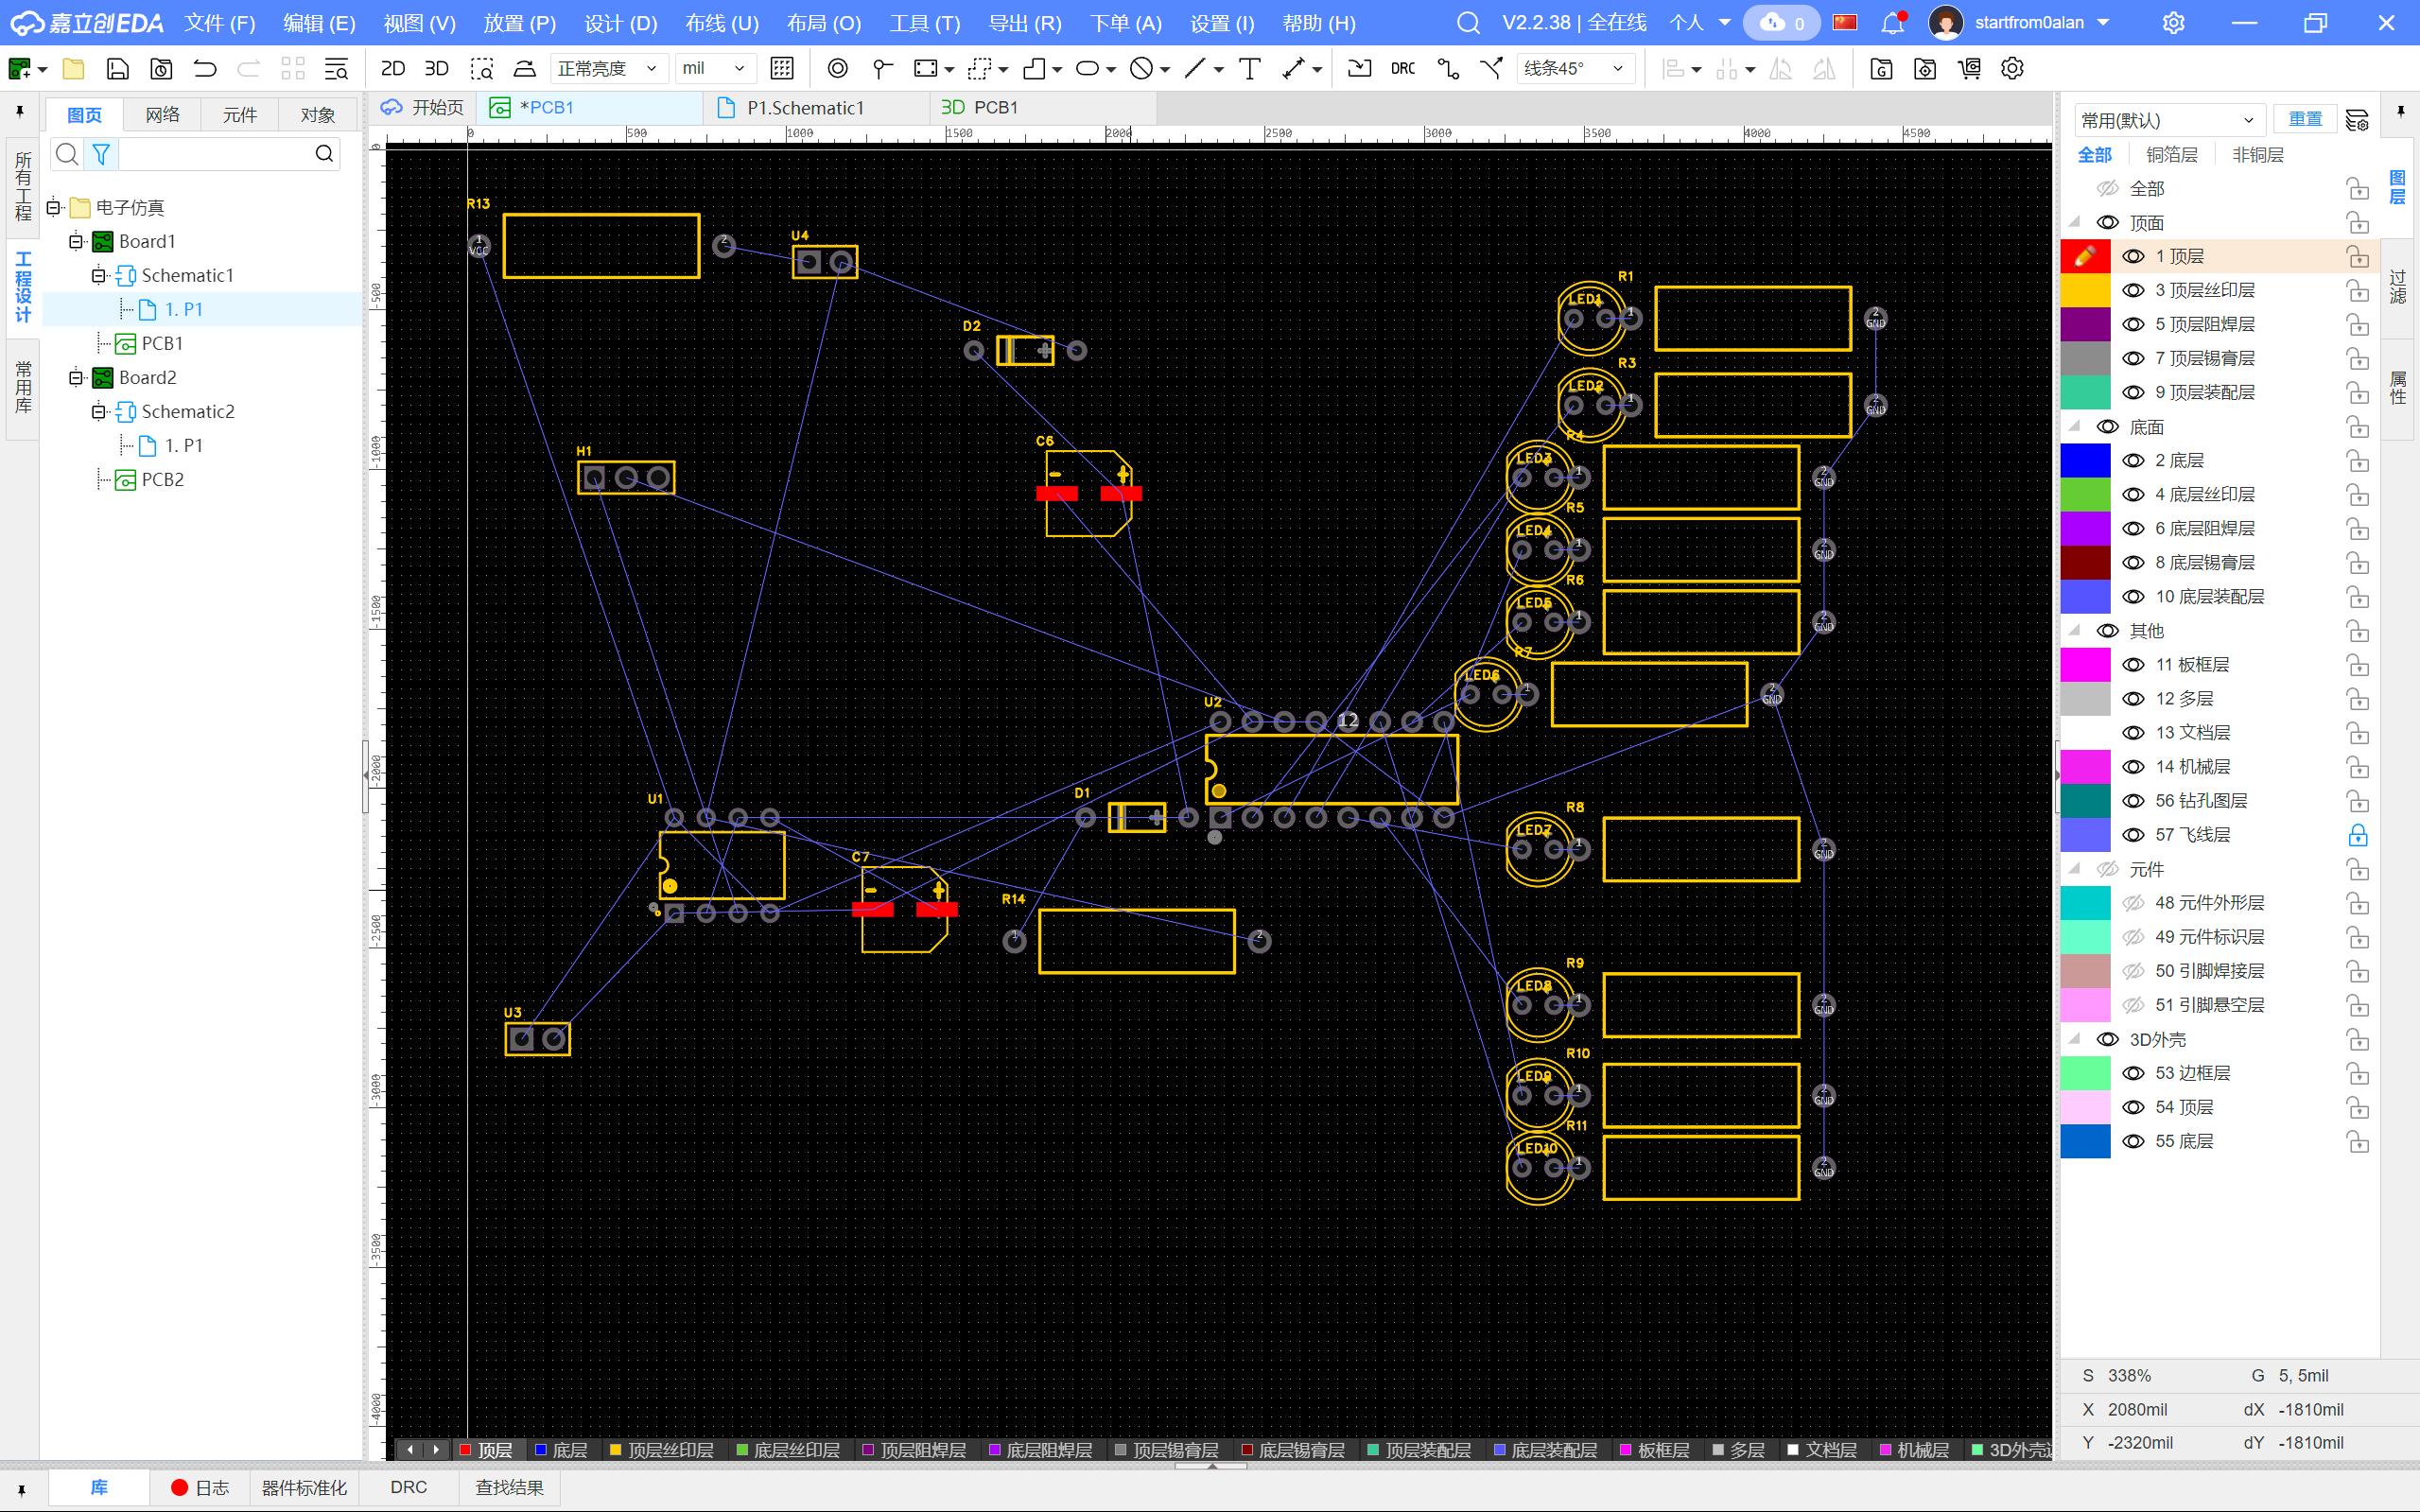
\includegraphics[width=0.85\textwidth]{pcb_2d.png}
    \caption{PCB 2D 效果图}
    \label{fig:pcb_2d}
\end{figure}

\subsection{3D 模型}

\begin{figure}[H]
    \centering
    % 请确保上传了 3D 渲染图，命名为 pcb_3d.png
    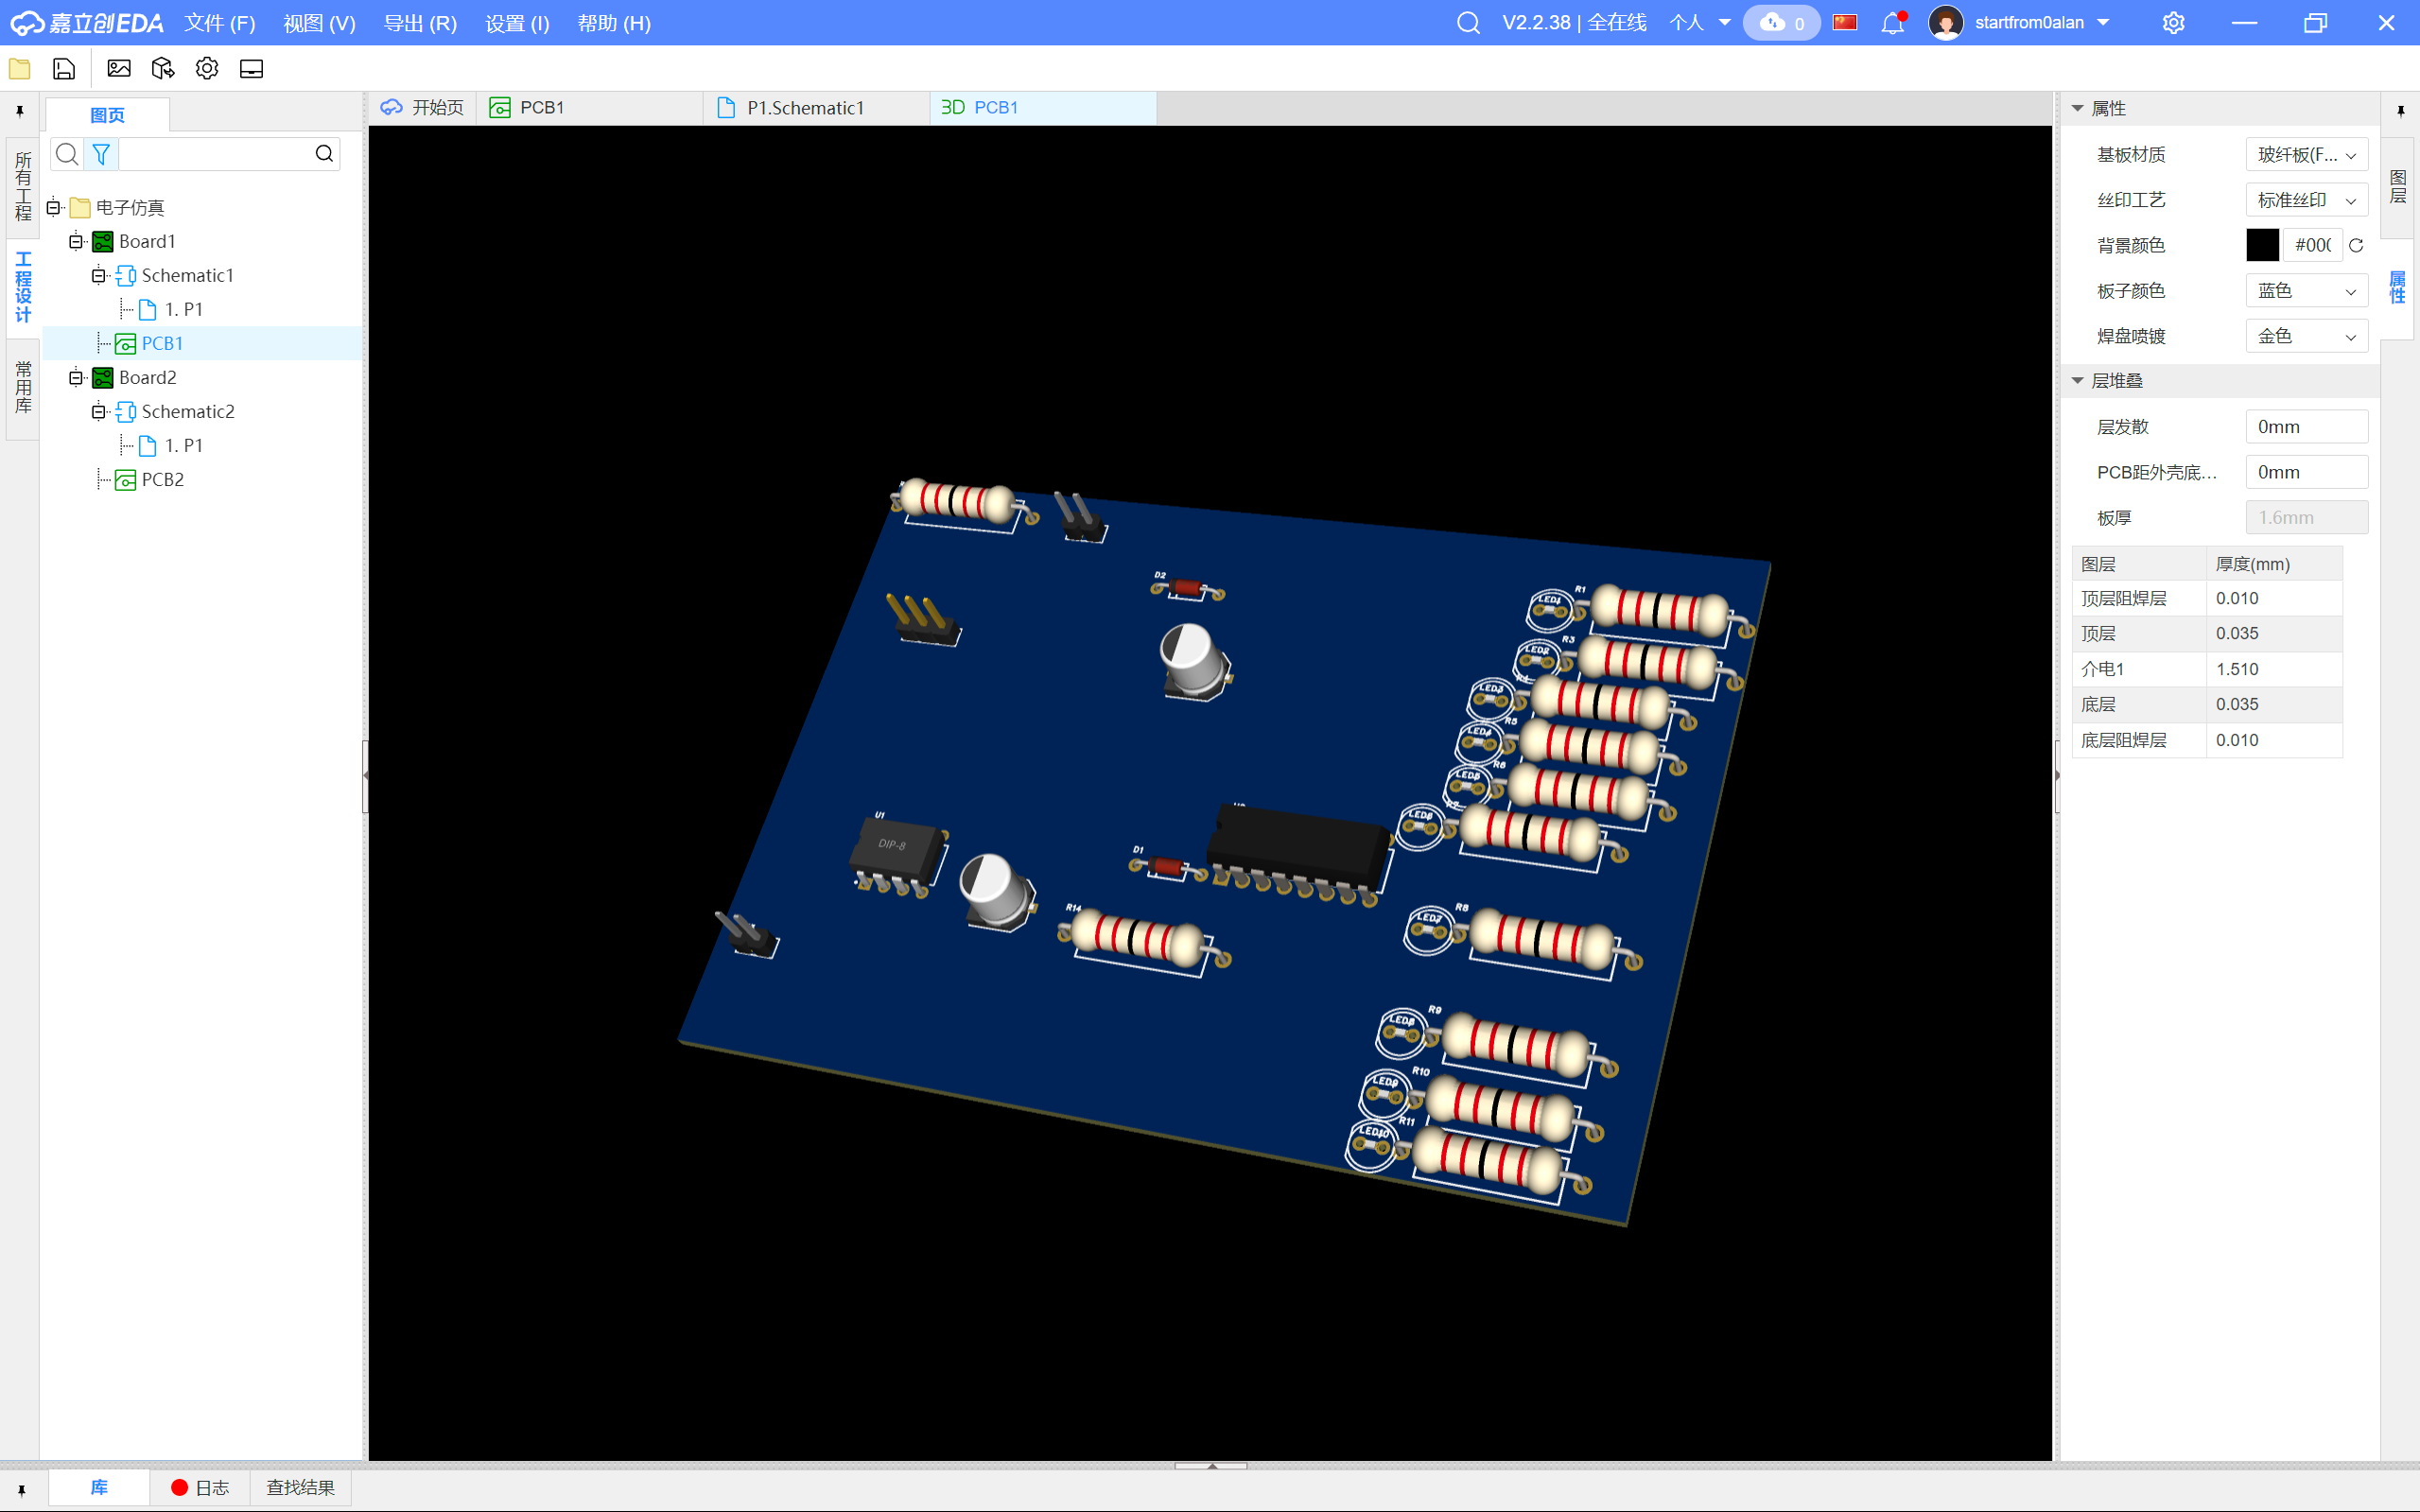
\includegraphics[width=0.85\textwidth]{pcb_3d.png}
    \caption{3D 渲染图}
    \label{fig:pcb_3d}
\end{figure}

\end{document}